% This is an article template

\documentclass[12pt]{article}

\usepackage{graphicx}
\usepackage[official]{eurosym}
\usepackage{color}
\usepackage{hyperref}
\graphicspath{ {./images/} }

\hypersetup
{   pdfauthor={van Deventer, Jan},
    pdfsubject={Indexed Line with IIoT},
    pdftitle={Sample document},
    pdfkeywords={LaTeX, PDF, hyperlinks}
}

\title{Indexed Line with IIoT}
\author{Aparajita Tripathy, Jan van Deventer \\Department of Computer Science, Electrical and Space Engineering\\Lule\aa\ Univerity of Technology \\ 971 87 Lule\aa, Sweden}
\date{\today}

\begin{document}
\maketitle

\begin{abstract}
This is a description of the functionality of a fischertechnik indexed line with two machining stations.
\end{abstract}

\section{Introduction}
% Introduction
The purpose of the ``Assembly Line''project is to have a public demonstrator that corroborates the potential of the open source Arrowhead Framework in an industrial IoT\footnote{Internet of Things.} automation setting.
Simultaneously, it  promotes knowledge transfer of the Arrowhead Framework as a documented example.

Physically, the assembly line is a fischertechnik ``toy'' developed for Industry 4.0 education \cite{fischertechnik}.
It is designated ``Indexed line with 2 machining stations 24\~V''\footnote{The documentation with that came with the assembly line can be found at the end of this document and includes a picture of the line.}.
It consists of two machining stations, a mill and a drill, where items are transported to each machine via conveyor belts.
The parts ``being'' machined are cylinders.
There are four conveyor belts:
\begin{enumerate}
 \item the loading conveyor belt, which receives the part and starts the whole process,
 \item the milling conveyor belt, which stops halfway to mill the part,
 \item the drilling conveyor belt, which stops halfway to drill the part.
 \item the offloading conveyor belt, which brings the part to be picked up and terminates the process.
\end{enumerate}
Conveyor belts 1 and 2, as well as 3 and 4 are at 90$^\circ$ from each other.
At each corner, a motorized slider pushes the part from one conveyor belt to the next and should then retract.
The conveyor belts have only one control signal, which is either on or off.
The motorized sliders have two exclusive\footnote{The PLC programmer should ensure not to have both directional requests at the same time.}  control signals: forward and backward,

To coordinate the conveyor belts, the sliders and the machining stations, nine sensors are available.
Four of sensors are switches associated with the motorized sliders to signal that they have reached their travel destinations.
That is each slider has two switches, one at each end.
When a slider moves forward, it should stop when it reaches the forward switch (I2 and I4 respectively)\footnote{Ix and Qx refer to the input and output pins of the circuit layout of the indexed line.}.
As soon as it stops in the forward position, it should retract (Q2 going low and Q1 going high for the first slider and Q4 going low and Q3 going high for the second slider) until it reaches its back switch (I1 and I3 respectively), at which point the slider should stop.
 
The loading conveyor belt (the first one) has two phototransistors (light beams, I7 and I5).
The phototransistor I7 indicates that a new item has been loaded onto the conveyor belt (and potentially increase the number of part being machined currently in the process).
The loading conveyor belt should start at that point (Q5 should be set high) and the belt moves at speed $v$ (cm/s).
When the item reaches the second phototransistor (I5), the milling conveyor belt should start (Q6).
After a delay $\Delta t_1$, the item should be in front of the first slider, and the slider should move forward (Q2 should be sent high).
This delay should be
\begin{equation} \label{eq:delay1}
 \Delta t_1 = \frac{d_1}{v}
\end{equation}
where $d_1$ is the distance in centimeters from the second phototransistor (I5) to the other side (or across) the milling conveyor belt.

The part or item shall then travel on the milling conveyor belt, and eventually cut the light beam of the third phototransistor (I6).
At that point, the milling conveyor belt should be stopped (Q6).
If the phototransistor is just under the milling machine, a small delay should be added (e.g., $r/v$, with $r$ being the radius of the item).
The milling machine (Q7 set high) should be turned on for 5 seconds, after which the milling conveyor belt should start again, as well as the drilling conveyor belt (Q8).

The item will travel all the way to the drilling machine phototransistor (I8), at which point both machining conveyor belts should stop (Q6 and Q8).
The drilling machine should be operated for 5 seconds (Q9).
The drilling conveyor belt should start again (Q8) as well as the offloading conveyor belt (Q10).
After a delay of $\Delta t_2$, calculated in a similar fashion as equation \ref{eq:delay1}, the second motor slider should move forward the item such that it is transferred to the final conveyor belt.
The drilling conveyor belt should be stopped (Q8).
The second slider will trip its forward switch (I3) at which time it should stop (Q4 going low) and return backwards (Q3 going high) until the back switch (I4) is tripped when the slider is stopped (Q3 going low).
As the item passes the last phototransistor (Q10), the final conveyor belt should be stopped. (If an item counter is used, it should be decremented.)


\section{Wiring}
% Wiring

There are two ways to connect the Indexed line to the PLC unit:
\begin{itemize}
  \item Using a 26 pin connector,
  \item Using the 24 wires that we can connect individually.
\end{itemize}
The table bellow shows how the 26 pin connector is connected to the PLC.

\begin{center}
\begin{tabular}{ |c|c|c|c| } 
 \hline
 Pin & Signal & PLC connection & Color \\ 
 \hline
  1 & +24V Actuators & NC & Brown \\ 
  2 & +24V Sensors & NC & Red \\ 
  3 & GND & NC & Orange \\ 
  4 & GND & DI 1 & Yellow \\ 
  5 & I1 & DI 1 & Green \\ 
  6 & I2 & DI 2 & Blue \\ 
  7 & I3 & DI 3 & Purple \\ 
  8 & I4 & DI 4 & Gray \\ 
  9 & I5 & DI 5 & White \\ 
  10 & I6 & DI 6 & Black \\ 
  11 & I7 & DI 7 & Brown \\ 
  12 & I8 & DI 8 & Red \\ 
  13 & I9 & DI 11 & Orange \\ 
  14 & NC & NC & Yellow \\ 
  15 & Q1 & DO 1 & Green \\ 
  16 & Q2& DO 1 & Blue \\ 
  17 & Q3 & DO 1 & Purple \\ 
  18 & Q4 & DO 1 & Gray \\ 
  19 & Q5 & DO 1 & White \\ 
  20 & Q6 & DO 1 & Black \\ 
  21 & Q7 & DO 1 & Brown \\ 
  22 & Q8 & DO 1 & Red \\ 
  23 & Q9 & DO 1 & Orange \\ 
  24 & Q10 & DO 1 & Yellow \\ 
  25 & GND & NC & Green \\ 
  26 & GND & NC & Blue \\ 
\hline
\end{tabular}
\end{center}

``DI'' stands for the Siemens Digital Input module and ``DO'' for the Digital Output module.
``NC'' indicates that there is no connection at that end of the wire.
The connection 9 and 10 on the PLC connectors are skipped since they can be used as linked connection between the left and right side of the connector.
The power and ground cables are not connected via the 26 pin connector because we had initially used the single wired inputs and no analysis was done to support the use of the thin wires to power the Indexed Line.

\section{Digital Twin}

\section{Plant Description}

\section{Arrowhead Services}
%It would be interesting to include a section describing the general approach followed to map the different signals/variables in the OPC-UA server to Services in an Arrowhead Local cloud.

%I do not know if this part needs to include details about how the OPC-UA server is configured, or is enough with the information about the services registered in the Service Registry. This last part is what I am most interested, such that an Arrowhead System can use the assembly line to manufacture a product.
The components in the assembly line (Sensors and Actuators) are integrated to Arrowhead cloud as services through the PLC's in-built OPC-UA server.Each of the input (Sensors) and output (Actuators) signals are declared as variables in the OPC-UA server which can be registered in the Arrowhead service registry as read and write services. In Figure  \ref{Figure 1.PNG}, the OPC-UA client contains 20 nodes, out of which 19 nodes refer to the signal values of sensor and actuator, whereas the last node is responsible for triggering the production process in factory.
\begin{figure}[h]
\caption{OPCUA Client}
\label{Figure 1.PNG}
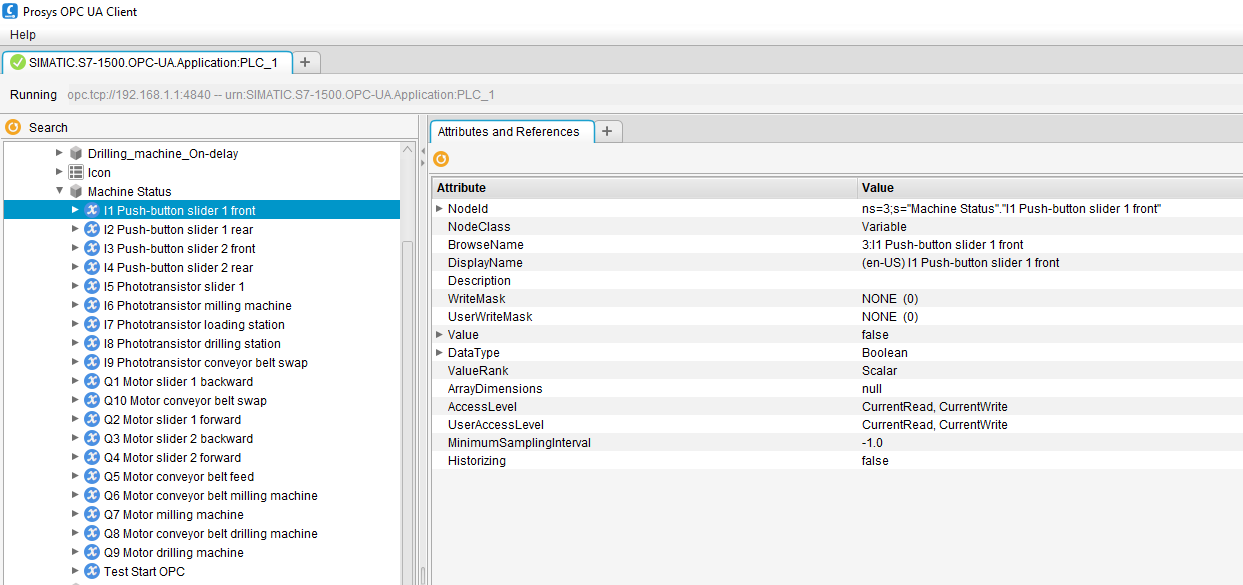
\includegraphics[width=12cm]{Documentation/assemblyLine/sections/Images/OPCUA_Variables.PNG}
\end{figure}

  The sensors and actuators are registering the below services in the Service Registry as illustrated in Figure 2 and 3.
  
  1. Sensors: One GET service, which is responsible for providing the status of the sensor signal (true/false).
  2. Actuators: Two services
        a) One GET service, which is responsible for providing the status of the actuator signal (true/false), 
        b) One POST service, which is responsible for changing the current status of the actuator signal.
  
\begin{figure}[h]
\caption{Arrowhead Services}
\label{Figure 2.PNG}
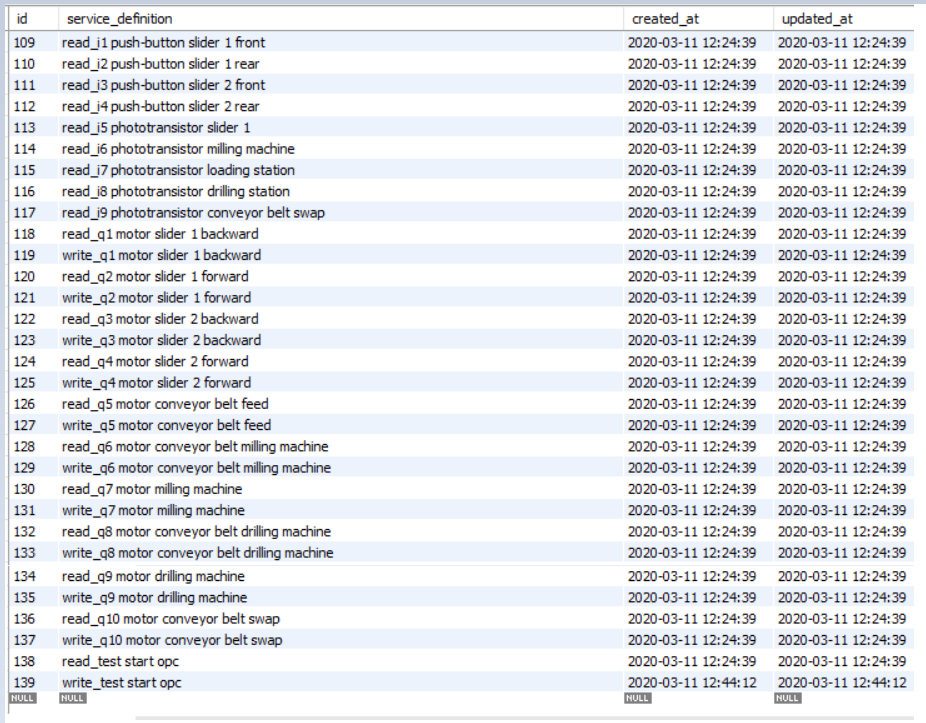
\includegraphics[width=12cm]{Documentation/assemblyLine/sections/Images/Service_Definitions.PNG}
\end{figure}

\begin{figure}[h]
\caption{Service Registry}
\label{Figure 3.PNG}
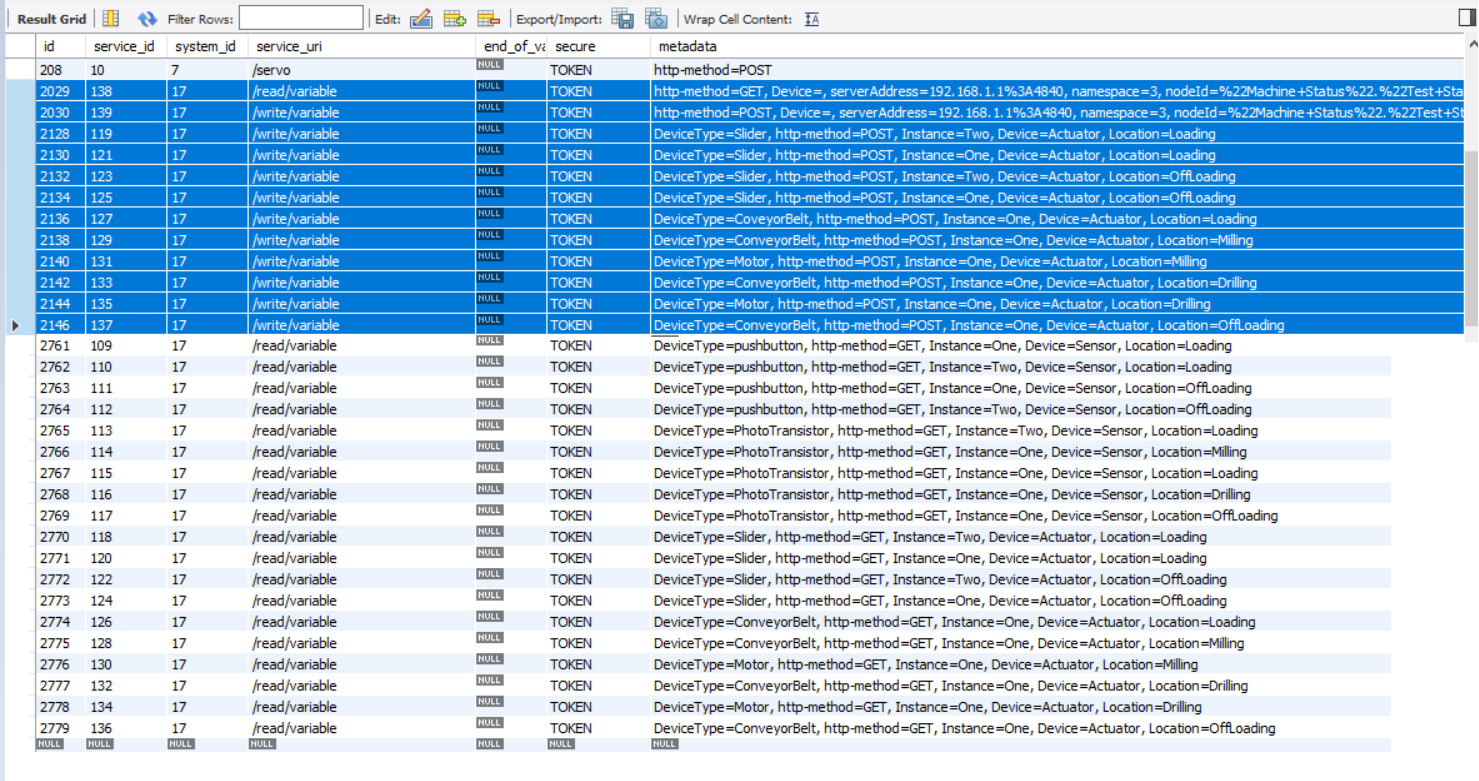
\includegraphics[width=12cm]{Documentation/assemblyLine/sections/Images/ServiceRegistry.png}
\end{figure}
%\end{document}

%\bibliographystyle{abbrv}
%\bibliography{bibFile}

\end{document}
  